\newpage
{\let\cleardoublepage\relax \chapter{Opis działania aplikacji}}
\label{cha:main}



\section{Proces nauczania}
Proces nauczania podzielony jest na 2 etapy :
\begin{itemize}
	\item Trening
	\item Powtórkę
\end{itemize}


\begin{center}
	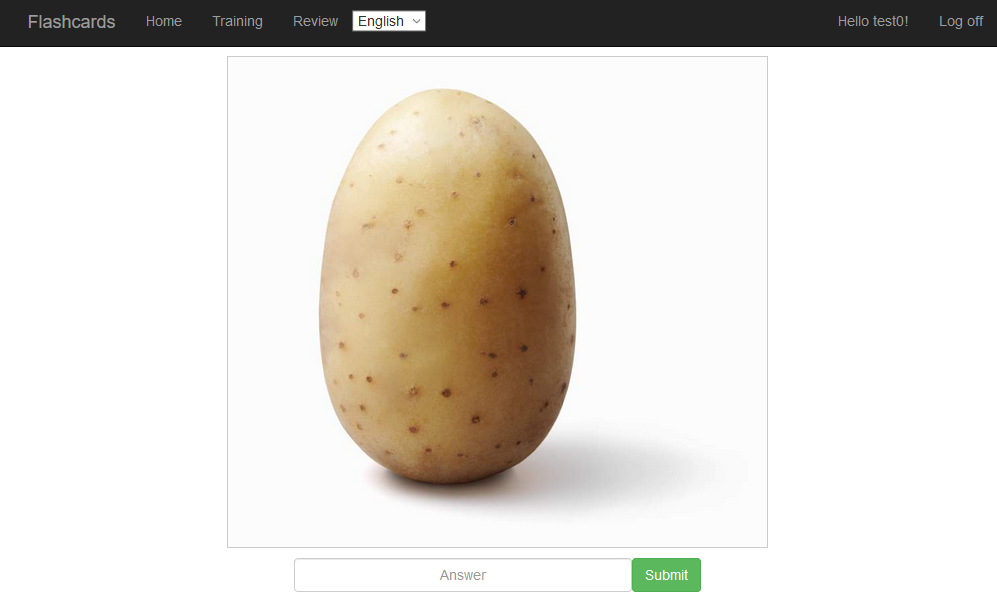
\includegraphics[width=\textwidth]{images/question.png}
	 \captionof{figure}{Widok pytania w projekcie. Jest on wspólny dla każdego z etapów}
\end{center}

\subsection{Trening}

W trakcie treningu użytkownik po raz pierwszy może spotkać się z danym słowem występującym w procesie nauki. Celem tego etapu jest zaznajomienie użytkownika z nowym słowem, zanim zacznie go używać w ramach powtórki.
Trening korzysta z kolejki, wewnątrz której znajduje się maksymalnie 5 fiszek. Tak mała ilość ma na celu łatwiejsze przyswojenie nowego materiału.

W przypadku poprawnej odpowiedzi na pytanie fiszka jest usuwana z kolejki i dodawana do zapamiętanych fiszek, w przeciwnym wypadku przechodzi na koniec kolejki zwiększając ilość niepoprawnych odpowiedzi o 1.

Ilość niepoprawnych odpowiedzi będzie decydować o wskaźniku siły dla danej fiszki po jej wstępnym nauczeniu.

\subsection{Powtórka}
\label{sub:powtorka}
W powtórce mogą wystąpić jedynie te fiszki, na które użytkownik odpowiedział poprawnie w trakcie treningu i ich interwał czasowy od ostatniego powtórzenia już minął. Ten etap także składa się z kolejki, lecz jest ona maksymalnie 30 elementowa. 

W przypadku poprawnej odpowiedzi na pytanie fiszka jest usuwana z kolejki i obliczany dla niej jest nowy interwał oraz siła z jaką jest zapamiętana. W przeciwnym wypadku fiszka jest przesuwana w pewne miejsce kolejki obliczane na podstawie poprzednich niepoprawnych odpowiedzi na tą fiszkę w danej powtórce. 

Na poniższej tabeli i obrazku można zobaczyć wewnątrz jakich zakresów znajdzie się wstawiana fiszka. Warto tutaj zaznaczyć iż 0 będzie oznaczała tutaj pierwsze miejsce w kolejce, zaś 1 będzie ostatnim miejscem w kolejce.
Dla przykładu jeśli fiszka ma zostać wstawiona między pozycją $\frac{1}{3}$ a $\frac{1}{2}$ i kolejka liczy aktualnie 20 kart. To zostanie ona wstawiona na pozycje 6,7,8,9, lub 10.

%\subsubsection{Miejsce w kolejce}

%Miejsce w którym fiszka znajduje się po niepoprawnej odpowiedzi jest obliczane tylko na podstawie ilości poprzednich niepoprawnych odpowiedzi i wygląda następująco:
%\begin{minipage}
%\newpage
\begin{center}
\begin{tabular}{| l | l | l |}
\hline
Ilość złych odpowiedzi  & Minimalna pozycja w kolejce & Maksymalna pozycja w kolejce \\ \Xhline{3\arrayrulewidth}

1 & $\frac{1}{3}$ & $\frac{1}{2}$   \\ \hline
2 & $\frac{1}{4}$  & $\frac{1}{3}$   \\ \hline
3 lub więcej & $\frac{1}{5}$   & $\frac{1}{4}$   \\ \hline
\end{tabular}
\captionof{table}{Miejsce w którym znajdzie się fiszka po niepoprawnej odpowiedzi w trybie powtórki}
\label{table:internals}

\end{center}
%\end{minipage}

\begin{center}
	\centering
	\includegraphics[width=\textwidth]{images/interval.png}
	 \captionof{figure}{Zobrazowanie informacji zawartych w tabeli \ref{table:internals}}
\end{center}
%\end{minipage}


\newpage
\subsection{Siła}

Siła jest atrybutem zapamiętanych fiszek dla danego użytkownika. Jest liczbą stałoprzecinkową z zakresu 0-1, gdzie 0 oznacza kompletnie nie zapamiętaną fiszkę, a 1 bardzo dobrze zapamiętaną.  \\
W przypadku poprawnej odpowiedzi na daną fiszkę siła jest obliczana na podstawie poniższych wzorów:  \\

\fbox{
 \addtolength{\linewidth}{-2\fboxsep}%
 \addtolength{\linewidth}{-2\fboxrule}%
 \begin{minipage}{\linewidth}
  \begin{align} \label{eq:winCorr}
   r(x) &= (1 - x^3) * corr \\ 
   \textnormal{Nowa siła} &= \frac{3x + r(x)}{3 + r(x)} \label{eq:winStr}
  \end{align}
 \end{minipage}
}

Gdzie:
\begin{itemize}
	\item x - aktualna ilość siły
	\item corr - Wskaźnik ważności danego tłumaczenia pomnożony przez poprawność wpisanego słowa.
\end{itemize}


\begin{center}
	\centering
	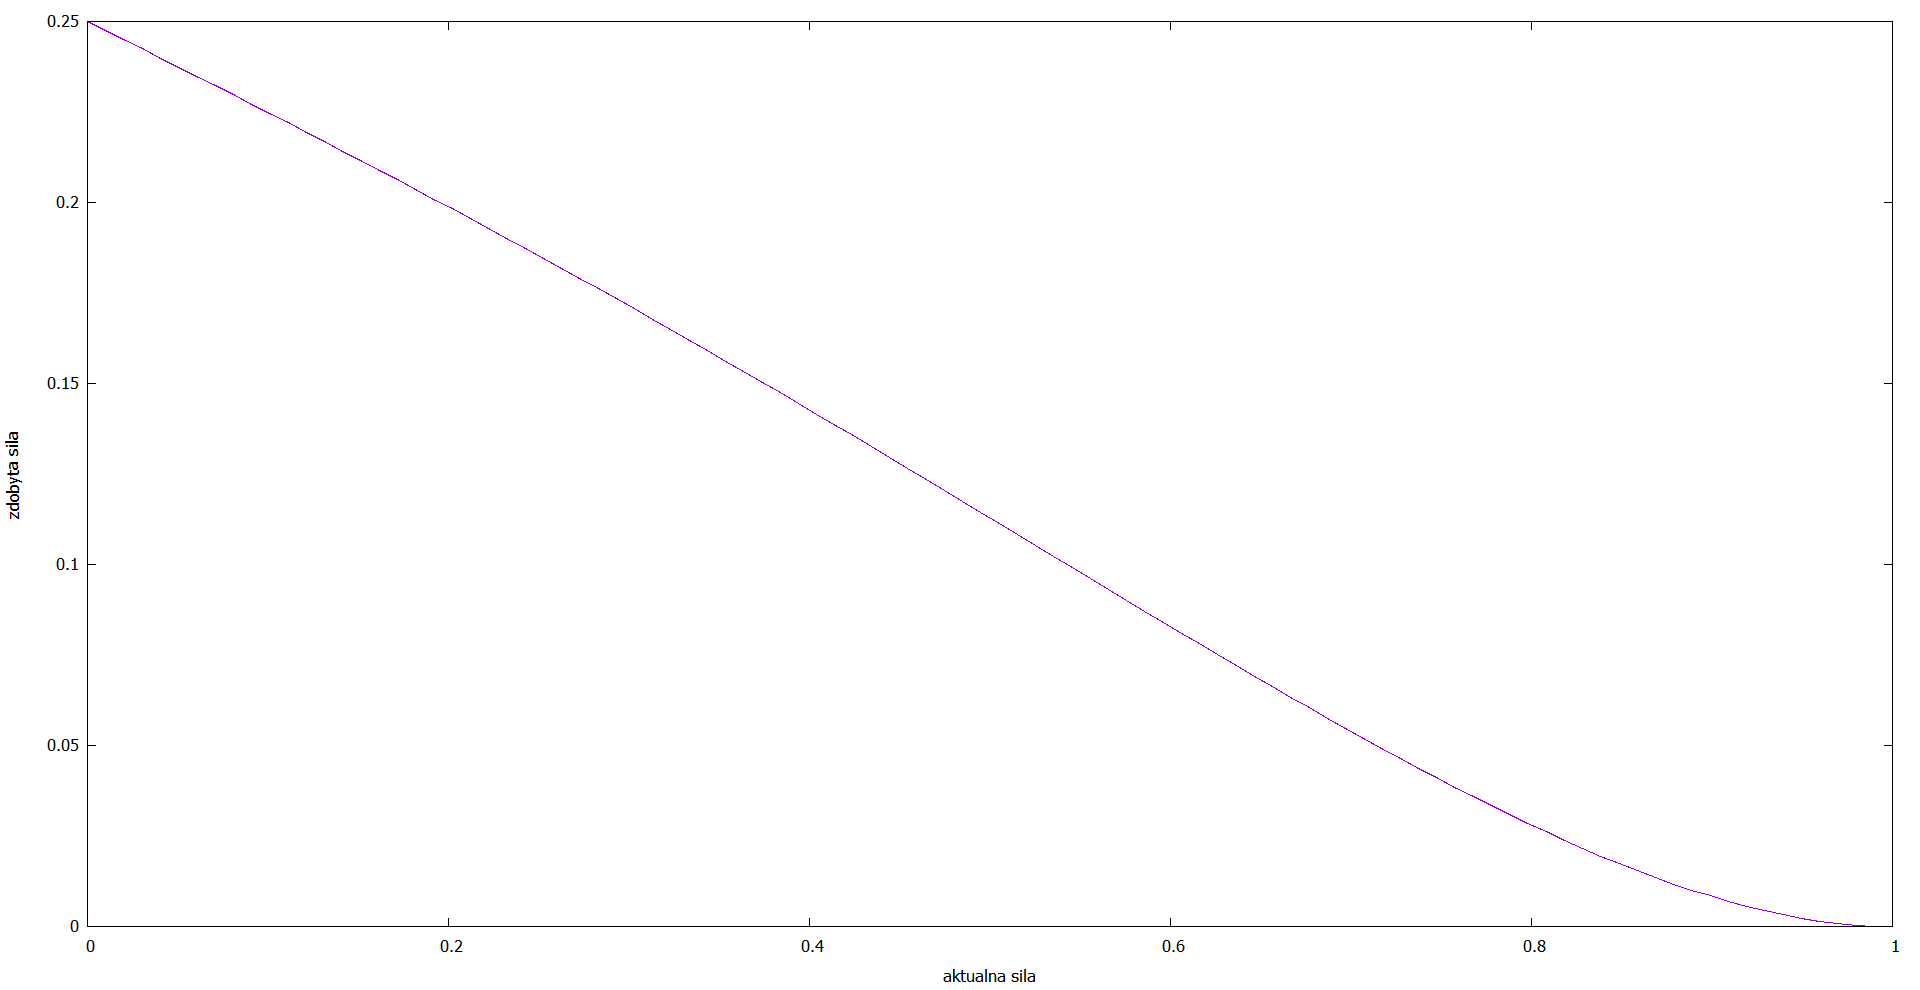
\includegraphics[width=\textwidth]{images/WinStrength.png}
	 \captionof{figure}{Wykres przedstawia ilość zdobytej siły po poprawnej odpowiedzi. Powstał na podstawie różnicy między nową siłą a jej poprzednią wartością.}
\end{center}

W przypadku poprawnej odpowiedzi na pytanie, które miało już przynajmniej 1 niepoprawną odpowiedź wzór na nową wartość siły wygląda następująco: \\

\fbox{
 \addtolength{\linewidth}{-2\fboxsep}%
 \addtolength{\linewidth}{-2\fboxrule}%
 \begin{minipage}{\linewidth}
  \begin{equation} \label{eq:lossStr}
  \textnormal{Nowa siła} = \frac{x}{L + x} 
  \end{equation}
 \end{minipage}
}

Gzie L oznacza ilość niepoprawnych odpowiedzi.

\begin{center}
	\centering
	\includegraphics[width=\textwidth]{images/LossStrength.png}
	  \captionof{figure}{Wykres przedstawia ilość straconej siły dla L = 1. Wzór \ref{eq:lossStr}.}
\end{center}

Wzór na siłę po zakończonym treningu dla danej fiszki wygląda następująco:\\

\fbox{
 \addtolength{\linewidth}{-2\fboxsep}%
 \addtolength{\linewidth}{-2\fboxrule}%
 \begin{minipage}{\linewidth}
  \begin{equation}
  \textnormal{Nowa siła} = \frac{0.5}{L + x} 
  \end{equation}
 \end{minipage}
}

\subsection{Interwały czasowe}

Pomiędzy kolejnymi wystąpieniami danej fiszki w trybie powtórki musi minąć ściśle określony interwał czasowy, który w zależności od poprawności odpowiedzi może maleć lub rosnąć. 
Interwał czasowy zawsze wyrażany jest w dniach. Pierwsze dwa interwały mają odpowiednio wielkość 1 i 6 dni.
\\
W przypadku poprawnej odpowiedzi na dane pytanie nowy interwał jest liczony według następującego wzoru:


\fbox{
 \addtolength{\linewidth}{-2\fboxsep}%
 \addtolength{\linewidth}{-2\fboxrule}%
 \begin{minipage}{\linewidth}
  \begin{align}  \label{eq:winInterval}
  I(n) &= \begin{cases}
  1 & \quad n = 1 \\
  6 & \quad n = 2 \\
  \left \lceil{I(n - 1) * (1 + x * \textnormal{factor})}\right \rceil  & \quad n \geq 3 \\
  \end{cases} \\ \label{eq:intervalFactor}
  \textnormal{factor} &= 1 - \frac{I(n - 1)}{30}
  \end{align}
 \end{minipage}
}

Gdzie:
\begin{itemize}
	\item I(n) - n-ty interwał
	\item x - Siła obliczona ze wzoru \ref{eq:winStr}
\end{itemize}

W przypadku poprawnej odpowiedzi poprzedzonej serią niepoprawnych odpowiedzi interwał jest liczony według następującego wzoru:


\fbox{
 \addtolength{\linewidth}{-2\fboxsep}%
 \addtolength{\linewidth}{-2\fboxrule}%
 \begin{minipage}{\linewidth}
  \begin{align} \label{eq:lossInterval}
  I(n) &= \left \lfloor{I(n - 1) * \frac{1 - x}{2}}\right \rfloor 
  \end{align}
 \end{minipage}
}

Gdzie x oznacza siłę liczoną według wzoru \ref{eq:lossStr}.

\subsection{Wykrywanie poprawności odpowiedzi}
\label{sec:similarity}
W celu określenia poprawności odpowiedzi używa się metryki, która w przedziale 0-1 określa podobieństwo dwóch wyrazów. Używana jest w tym celu odległość Levenshteina określająca odległość między dwoma wyrazami na podstawie najmniejszej ilości operacji prostych jakie są potrzebne, aby przekształcić jeden wyraz w drugi. \cite{Leve}

Operacja prosta może być:
\begin{itemize}
	\item Usunięciem danego znaku
	\item Wstawieniem nowego znaku
	\item Zamianą danego znaku na inny
\end{itemize}

W celu uzyskania miary podobieństwa wyrazów używa się poniższego wzoru: 

\fbox{
 \addtolength{\linewidth}{-2\fboxsep}%
 \addtolength{\linewidth}{-2\fboxrule}%
 \begin{minipage}{\linewidth}
  \begin{align} 
  L &= {\frac{|s_1| + |s_2|}{2}}^{1.1} \\
  \textnormal{Podobieństwo} &= \frac{L - D}{L} \label{eq:distance}
  \end{align}
 \end{minipage}
}

Gdzie :
\begin{itemize} 
	\item $s_1$, $s_2$ - wyrazy które porównujemy
	\item D - dystans Levenshteina
\end{itemize}

\vspace{1cm}

Odpowiedź jest poprawna, jeśli:
\begin{itemize}
	\item Ma podobieństwo większe niż 0.82 dla trybu treningowego.
	\item Ma podobieństwo większe niż 0.7 w trakcie powtórki.
\end{itemize}

\subsection{Możliwe odpowiedzi}

Każda fiszka dla danego języka ma zestaw tłumaczeń, które definiują możliwy zbiór poprawnych odpowiedzi. Każde tłumaczenie składa się z:
\begin{itemize}
	\item Poprawnej odpowiedzi.
	\item Zapisu fonetycznego.
	\item Ważności tłumaczenia, która jest używana we wzorze \ref{eq:winCorr}.
\end{itemize}
W trakcie udzielania odpowiedzi na pytanie, wybierane jest to tłumaczenie, które ma największą miarę podobieństwa (\ref{eq:distance}) wśród tłumaczeń dla danej fiszki.

\subsection{Obrazki}

Każda fiszka musi zostać zaopatrzona w odpowiedni zestaw obrazów, z których jeden z nich zostanie wylosowany do procesu sprawdzenia wiedzy użytkownika. Ważne jest, aby obrazki jak najlepiej oddawały przedstawiane słowo i były jak najbardziej zróżnicowane.

\subsection{Dostosowanie wzorów}

W poprzednich podrozdziałach pojawiły się wzory związane z interwałami oraz siłą. Wzory \ref{eq:winStr}, \ref{eq:lossStr}, \ref{eq:winInterval}, \ref{eq:intervalFactor} i \ref{eq:lossInterval} powstały na zasadzie zdefiniowania sparametryzowanych równań, których parametry były dobierane na zasadzie znalezienia najlepszego ich zestawu na podstawie symulacji. Do symulacji były dobierane skończone zestawy parametrów z przestrzeni rozwiązań.

Na potrzeby symulacji powstały następujące równania:


\fbox{
 \addtolength{\linewidth}{-2\fboxsep}%
 \addtolength{\linewidth}{-2\fboxrule}%
 \begin{minipage}{\linewidth}
  \begin{align} 
  L &= {\frac{|s_1| + |s_2|}{2}}^{1.1} \\
  \textnormal{Podobieństwo} &= \frac{L - D}{L} \label{eq:distance}
  \end{align}
 \end{minipage}
}

\todo[inline]{Dorobić tutaj właściwe wzory. Ale to dopiero w domu}

Wzory [1],[2],[3],[4] są odpowiednio odpowiednikami wzorów  \ref{eq:winStr}, \ref{eq:lossStr}, \ref{eq:intervalFactor} i \ref{eq:lossInterval}. Dla każdej ze zmiennych został określony przedział zmienności w jakim mogą się one zmieniać. Został on określony następująco:

\fbox{
 \addtolength{\linewidth}{-2\fboxsep}%
 \addtolength{\linewidth}{-2\fboxrule}%
 \begin{minipage}{\linewidth}
  \begin{align} 
   1 &\leq A \leq 9 \\
   0.25 &\leq B \leq 12 \\
   0.25 &\leq C \leq 10 \\
   0.25 &\leq D \leq 5 \\
   20 &\leq E \leq 50 \\
  \end{align}
 \end{minipage}
}

Zmienne A,B,C,D i E przyjmują zestaw wartości ze swoich przedziałów. Wartości, które przyjmują są od siebie równoodległe. T.j każda następna wartość była osiągana poprzez zinkrementowanie poprzedniej o stałą wartość dla danej zmiennej.

Zmienna E zawierała wszystkie liczby całkowite ze swojego przedziału.
\vspace{5mm}


Dla każdego zestawu zmiennych została przeprowadzona symulacja, która polegała na stworzeniu wirtualnego ucznia, który przez 360 dni poświęcał 60 minut na nauczenie się fiszek. Każda próba odpowiedzi na daną fiszkę powodowała utratę 1 minuty na naukę co w efekcie dawało uczniowi możliwość przeglądnięcia 60 fiszek danego dnia. Następnie uczeń wracał do nauki dokładnie po 24 godzinach. Z powyższego wynika fakt, iż między dwoma kolejnymi rozpoczęciami powtórek mijało 25 godzin.

Co więcej, uczeń każdego dnia dostawał 5 nowych fiszek do swojego zestawu fiszek, których się uczył.

Wynikiem symulacji jest ilość nauczonych fiszek, które miały przynajmniej 5 powtórzeń i są zapamiętane przez ucznia na poziomie przynajmniej 75\%. Celem jest znalezienie takiego zestawu wartości zmiennych, który zmaksymalizuje ten wynik.

\subsection{Wirtualny uczeń}

Wirtualny uczeń potrafi zapamiętywać informację zgodnie z krzywą zapominania. Uczeń wraz z biegnącym czasem traci szansę na poprawną odpowiedź na daną fiszkę. Procentowa szansa na odpowiedź jest obliczana na podstawie wzoru:

\fbox{
 \addtolength{\linewidth}{-2\fboxsep}%
 \addtolength{\linewidth}{-2\fboxrule}%
 \begin{minipage}{\linewidth}
  \begin{align} 
   R = \displaystyle e\strut^{\displaystyle \frac{-t}{s}}
  \end{align}
 \end{minipage}
}

Gdzie:
\begin{itemize}
\setlength\itemsep{1mm}
	\item t - czas od ostatniego zobaczenia danej fiszki.
	\item s - Ilość zobaczeń danej fiszki + 1.
\end{itemize}

Uznajemy, iż uczeń po zobaczeniu fiszki w odstępie czasu wynoszącym $t = 0$ ma 100\% szansę na poprawną odpowiedź. 
Zmienna czasowa zawiera tutaj ilość dni, które upłynęły od ostatniego powtórzenia. Więc $t = 1$ oznacza, iż od ostatniego powtórzenia upłynął 1 dzień.

\subsection{Wyniki symulacji}
W wyniku przeprowadzonych symulacji udało się uzyskać poniższy zestaw zmiennych:


\fbox{
 \addtolength{\linewidth}{-2\fboxsep}%
 \addtolength{\linewidth}{-2\fboxrule}%
 \begin{minipage}{\linewidth}
  \begin{align} 
   A &= \\
   B &= \\
   C &= \\
   D &= \\
   E &= 
  \end{align}
 \end{minipage}
}

\section{Narzędzia administratorskie}

Administrator posiada dodatkowe narzędzia, które pozwalają mu na :
\begin{itemize}
	\item Przeglądanie wszystkich fiszek.
	\item Dodanie nowej fiszki do systemu.
	\item Edycja danej fiszki - dodanie lub edycja tłumaczeń, dodanie lub usunięcie powiązanych obrazków.
\end{itemize}
Prawa administratorskie nadaje się poprzez nadanie roli administratora w tabeli \textbf{AspNetUserRoles}. Aktualnie należy użyć zapytania SQL, aby takowe uprawnienia nadać. 

\begin{center}
	\centering
	\includegraphics[width=\textwidth]{images/Management.png}
	  \captionof{figure}{Widok edycji fiszki.}
\end{center}


\section{Diagram przypadków użycia}

\begin{center}
	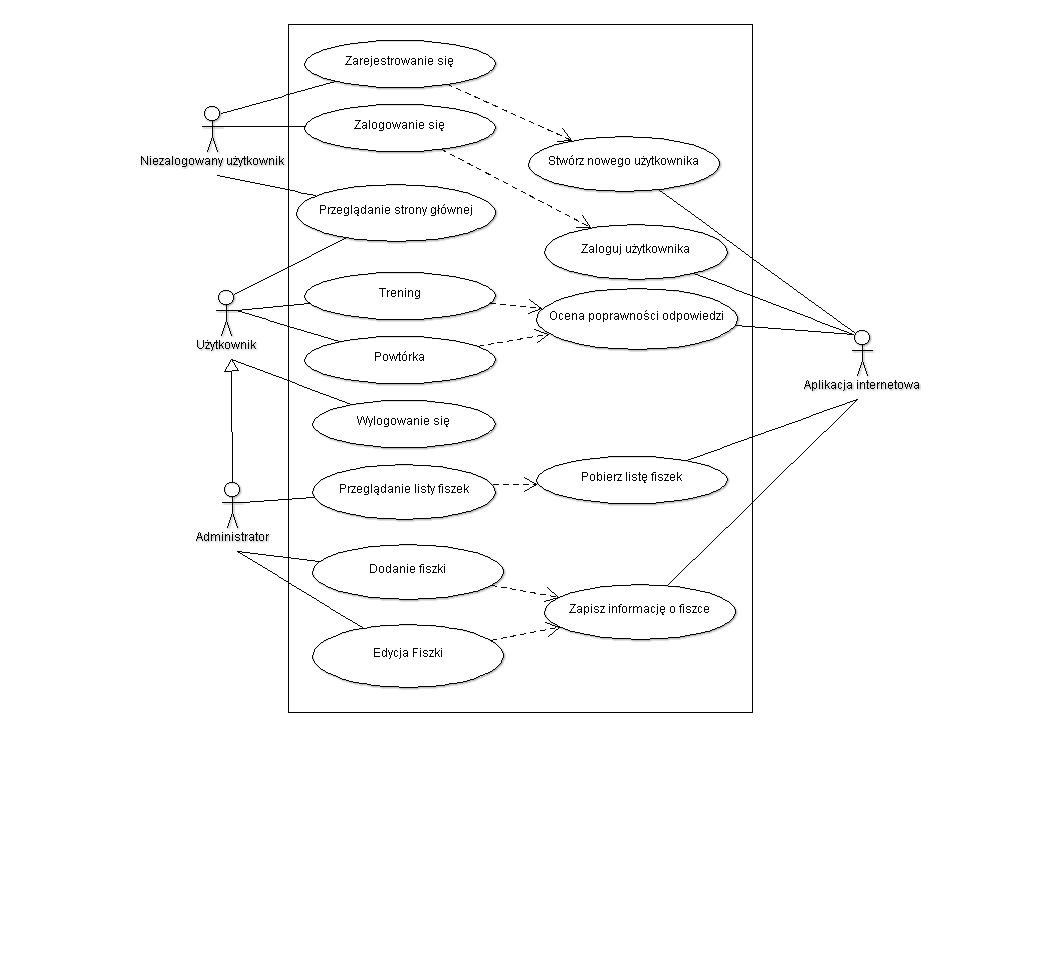
\includegraphics[width=\textwidth]{images/usecases.png}
	 \captionof{figure}{Diagram przypadków użycia.}
\end{center}


\newpage
{\let\cleardoublepage\relax \chapter{Kwestie techniczne}}

\section{Struktura programu}

\begin{center}
	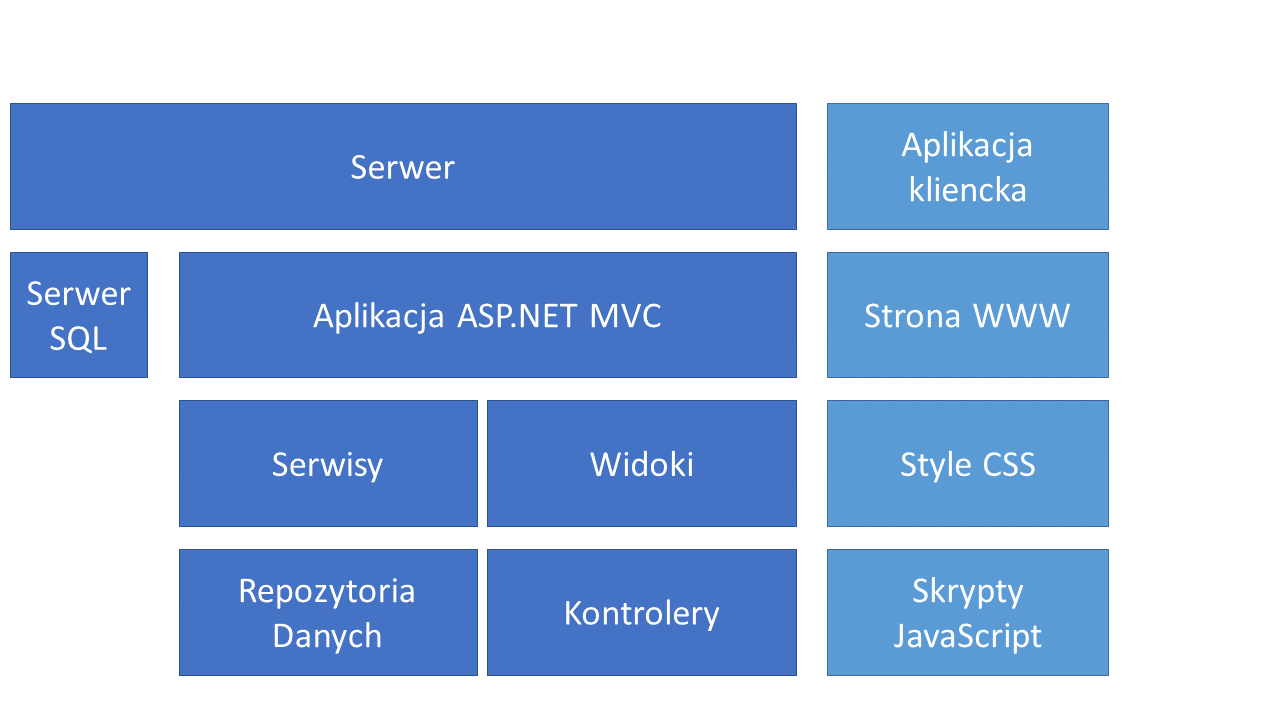
\includegraphics[width=\textwidth]{images/Structure.png}
	 \captionof{figure}{Diagram przedstawiający strukturę programu.}
\end{center}


\subsection{Repozytoria}

Repozytoria odpowiadają za dostęp do bazy danych(\ref{section_Repo}). Zawierają wewnątrz siebie kontekst do bazy danych, który pochodzi z frameworka Entity Framework. Dostarcza on metody operacji na bazie poprzez dostarczenie obiektu typu \textbf{DbSet<T>}, który umożliwia wykonanie zapytań na bazie danych. RepositoryBase implementuje wszystkie operacje, które są potrzebne w trakcie pracy z bazą danych. Klasy po nim dziedziczące wykorzystują metody bazowe w celu stworzenia bardziej skomplikowanych zapytań skonstruowanych pod daną tabelę zgodnie z wymaganiami biznesowymi. 

\begin{minipage}{\linewidth}
\begin{lstlisting}[
frame=single, numbers=none,captionpos=b, 
caption={Część implementacji RepositoryBase}]
public class RepositoryBase<TEntity, TContext> : RepositoryBaseEntityless<TContext>, IRepository<TEntity>, IDisposable
	where TEntity : class, new()
	where TContext : DbContext, new()
{
protected DbSet<TEntity> dbSet;

public DbSet<TEntity> DbSet { get { return dbSet; } }

public virtual IQueryable<TEntity> Query { get { return dbSet.AsQueryable(); } }

public RepositoryBase(TContext context) : base(context)
{
	dbSet = context.Set<TEntity>();
}
/*
Reszta metod wewnątrz których realizowany jest dostęp do danych
*/
}
\end{lstlisting}
\end{minipage}

\begin{landscape}
\begin{center}
	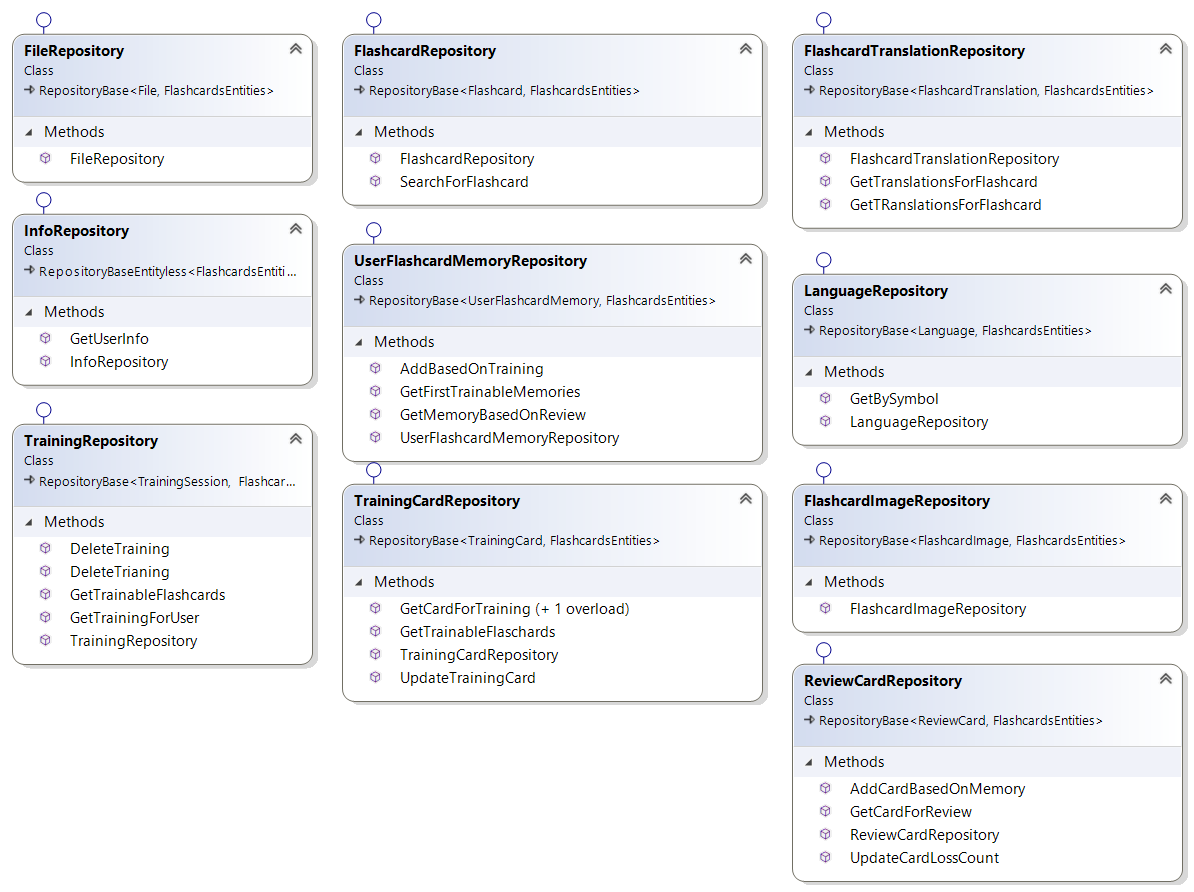
\includegraphics[width=\textwidth]{images/Repos.png}
	 \captionof{figure}{Diagram klas wszystkich repozytoriów w projekcie.}
\end{center}
\end{landscape}


\subsection{Kontrolery}

Kontrolery odpowiadają za wygenerowanie odpowiedzi dla danych zapytań. Wszystkie kontrolery wewnątrz aplikacji dziedziczą po klasie \textbf{ControllerBase}, która kolei dziedziczy po klasie \textbf{Controller}. ControllerBase odpowiada za zdefiniowanie wspólnych akcji jakie mogą być wykonywane przez wszystkie kontrolery. Ma to na celu zmniejszenie redundancji kodu jak i zwiększenie jego czytelności.

\begin{minipage}{\linewidth}
\begin{lstlisting}[
frame=single, numbers=none,captionpos=b, 
caption={Część implementacji ControllerBase}]
public class ControllerBase : Controller
{
	private readonly IPopupService popupService;
	protected readonly ISessionService sessionService;

	public ControllerBase(IPopupService popupService, ISessionService sessionService)
	{
		this.popupService = popupService;
		this.sessionService = sessionService;
	}
	 public ActionResult RedirectBackWithError(string errorMessage = "Error")
	{
		AddError(errorMessage);
		return RedirectBack();
	}
	/*Reszta metod zaimplementowanych przez ControllerBase*/
}
\end{lstlisting}
\end{minipage}

Każdy kontroler zawiera zestaw akcji, które wykonywane są w wyniku zapytań użytkownika i zwracają obiekt typu \textbf{ActionResult}. W zależności od tego jaki typ ma obiekt zwracany dana akcja potrafi:

\begin{itemize}
	\item wyrenderować stronę HTML.
	\item zwrócić skrypt JavaScript.
	\item Zwrócić informację zapisane w formacie JSON.
\end{itemize}

Dodatkowo, jeśli dana akcja ma zwrócić widok HTML to musi być dla niej zdefiniowany specjalny plik .cshtml, w którym znajduje się kod możliwy do wyrenderowania przez aktualny silnik renderujący. 
Metody dla akcji potrafią przyjmować argumenty, do których wartości przypisywane są na podstawie parametrów przekazanych w zapytaniu od użytkownika. 
\begin{landscape}
\begin{center}
	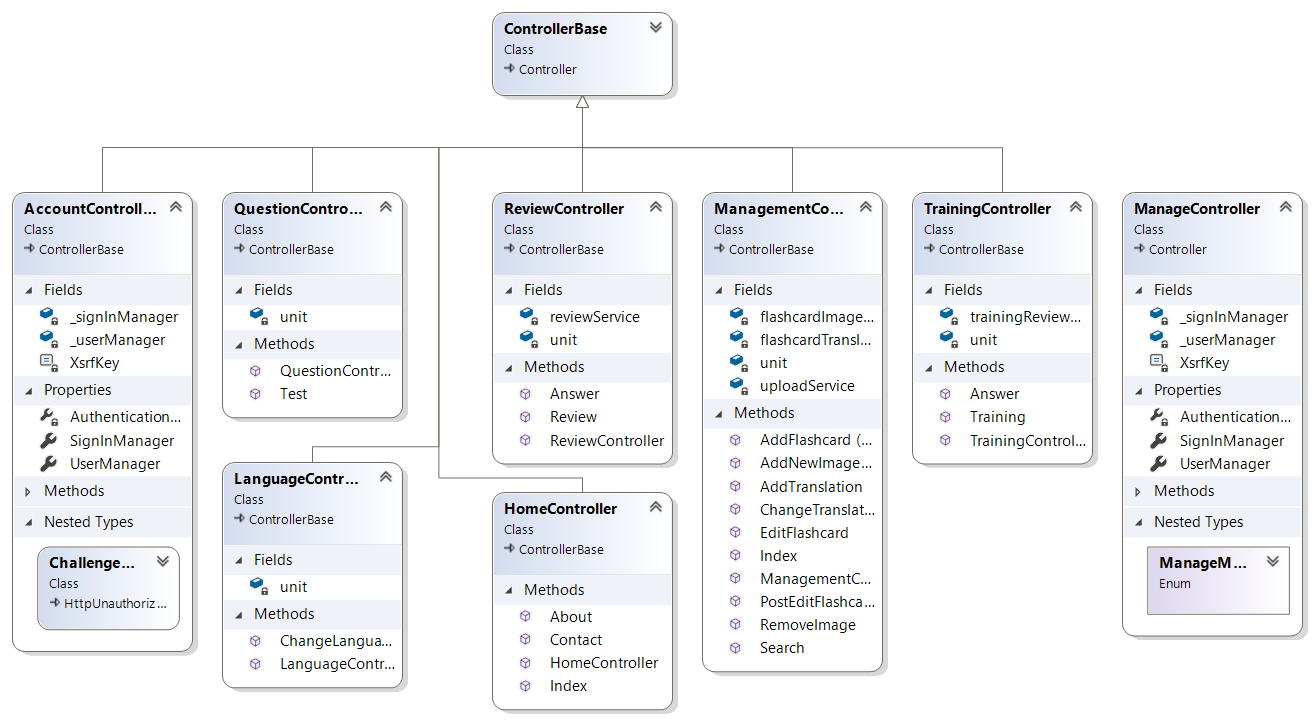
\includegraphics[width=\paperwidth]{images/Controllers.png}
	 \captionof{figure}{Diagram klas wszystkich kontrolerów w projekcie}
\end{center}
\end{landscape}

\subsubsection{Cykl życia kontrolera}

Cykl życia kontrolera składa się z 5 etapów:
\begin{itemize}
	\item Kreacji
	\item Autoryzacji i autentykacji.
	\item Bindowania wartości do modelu.
	\item wywołania odpowiedniej akcji
	\item zwrócenie rezultatu działania (\textbf{ActionResult})
\end{itemize}

\begin{center}
	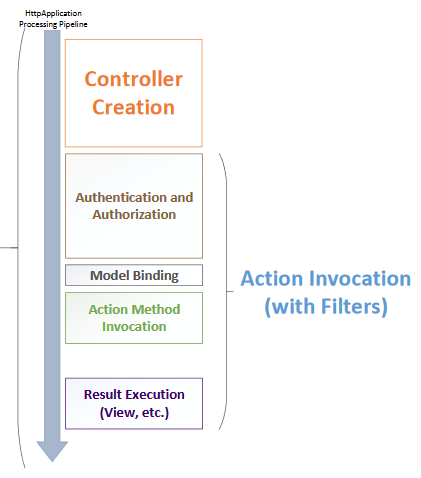
\includegraphics{images/ControllerLifecycle.png}
	 \captionof{figure}{Cykl życia kontrolera. Źródło: docs.microsoft.com.}
\end{center}

Na początku aplikacja musi określić jaki kontroler należy powołać do życia w celu obsługi zapytania. W tym celu są wykorzystywane tabele routingu, które mapują dane adresy URI na odpowiedni kontroler. 

Dla przykładu: Domyślnie adres URI localhost:25388/Home/Index zostanie zmapowany na HomeController, który wykonuje akcje Index.

Następnie \textbf{DependencyResolver} stara się utworzyć instancje danego kontrolera. Gdyby nie było DependencyResolvera, bądź zwróciłby on null w wyniku swojego działania to zostaje stworzony kontroler na podstawie jego bezparametrowego publicznego konstruktora. Jeśli takowego by nie było to rzucany jest wyjątek. Po utworzeniu kontrolera aplikacja stara się zbadać prawa do danego zasobu na podstawie wewnętrznych reguł i atrybutów przypisanych do danej akcji i kontrolera. Jeśli zdarzy się sytuacja w której użytkownik nie ma praw do danego zasobu to zostaje przekierowany na odpowiednią stronę błędu 401 lub 403.
\todo[inline]{Opisać bardziej atrbuty i reguły?}

Kolejnym krokiem jest zbindowanie możliwie jak największej ilości parametrów przekazanych w zapytaniu do argumentów metody, która po tym zabiegu zostanie wywołana.

Na samym końcu następuje zwrócenie rezultatu działania akcji, który zostaje zwrócony użytkownikowi.

\subsection{Serwisy}

Serwisy zawierają w sobie implementacje całej logiki biznesowej. Zostały podzielone w celu logicznego pogrupowania różnych operacji wykonywanych przez aplikację. Dla przykładu \textbf{StrengthService} służy jedynie do obliczania siły na podstawie wzorów \ref{eq:lossStr} i \ref{eq:winStr}.
\newpage

\begin{landscape}
\begin{center}
	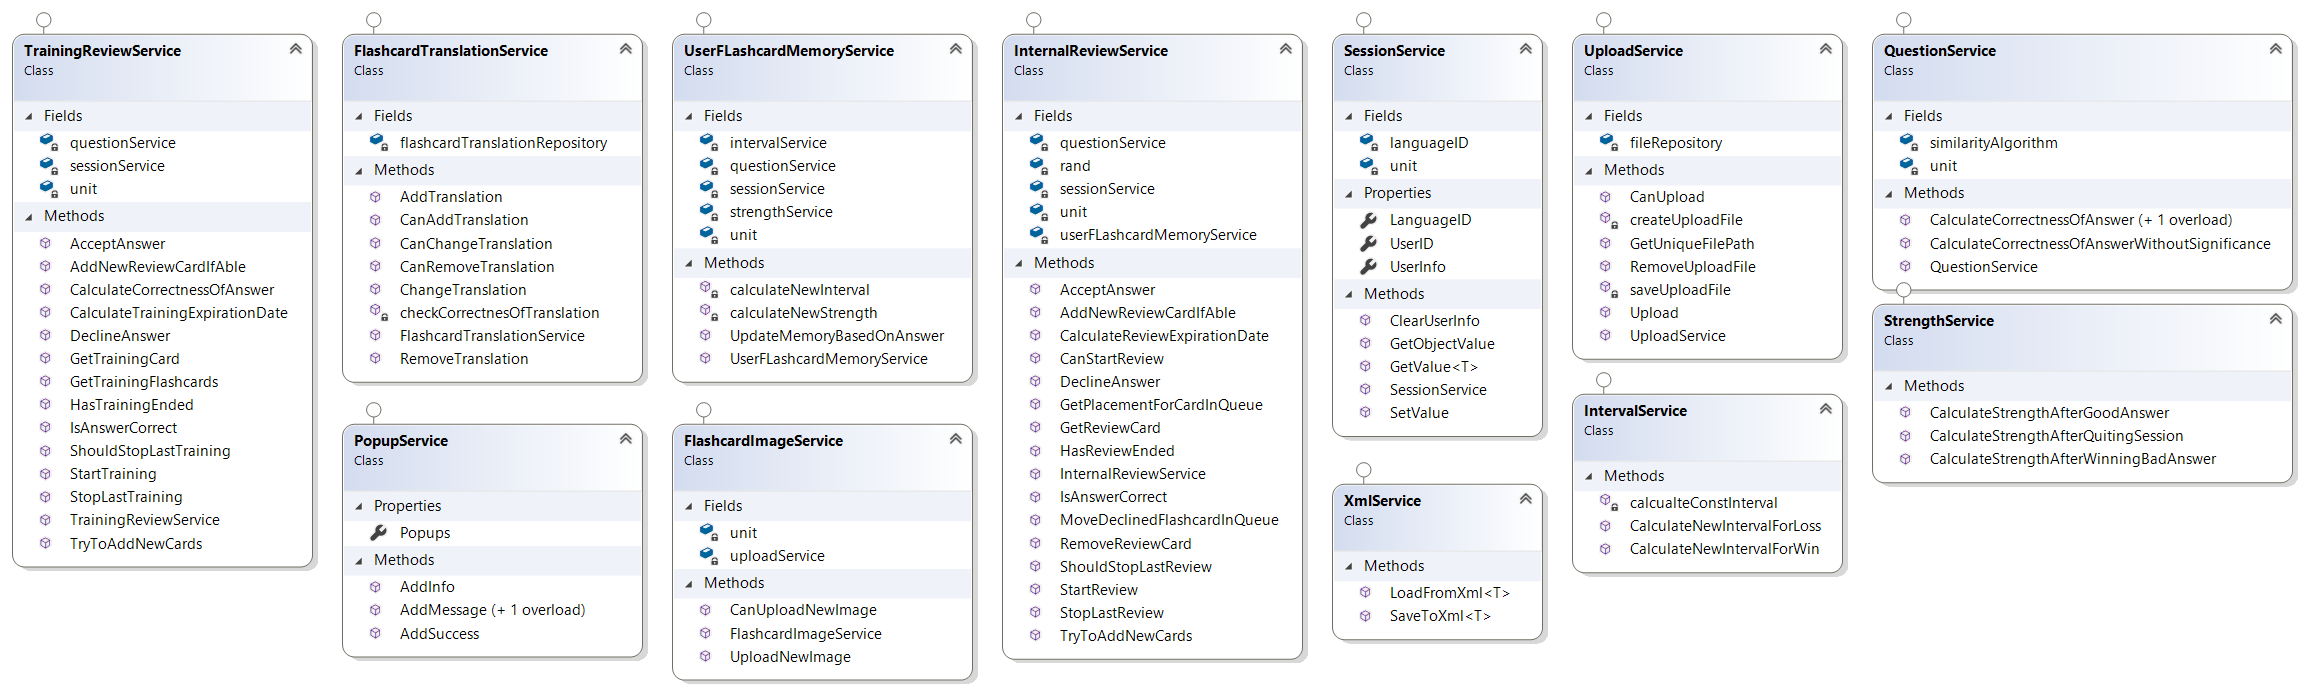
\includegraphics[width=\paperwidth]{images/Serwisy.png}
	 \captionof{figure}{Diagram klas wszystkich serwisów w projekcie}
\end{center}
\end{landscape}


\section{Struktura rozwiązania}

Rozwiązanie jest podstawową jednostką pracy wewnątrz programu Visual Studio. Zawiera w sobie wszystkie projekty, ich ustawienia, informację o kolejności ich kompilacji oraz dodatkowe pliki niezwiązane z żadnym projektem. Projekt posiada solucję, w której w skład wchodzi:

\begin{itemize}
	\item Projekt Common - zawierający metody ogólnego przeznaczenia.
	\item Projekt Entities - wykorzystujący wzorzec repozytorium. Służy do łączenia się z bazą danych.
	\item Projekt FlashcardCommon - zawierający metody związane z całym projektem.
	\item IntegrationTests - zawiera testy integracyjne.
	\item UnitTests - zawiera testy jednostkowe.
	\item TestSuite - zawiera zestaw narzędzi wykorzystywany przez testy. 
	\item Utilities - zawiera metody ogólnego przeznaczenia. 
	\item WebUtils - zawiera metody ogólnego przeznaczenia dla środowiska ASP.NET MVC.
	\item Management - zawiera porzuconą okienkową aplikacje administratora.
	\item Services - zawiera wszystkie serwisy wykorzystywane przez projekt.
	\item Flashcards - zawiera właściwą aplikację internetową.
	\item wirtualny folder git - zawiera w sobie pliki związane z repozytorium git\footnote{Repozytorium git służy do wersjonowania kodu.}.
\end{itemize}

\begin{center}
	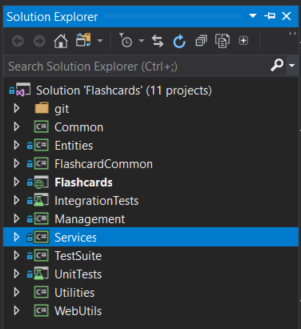
\includegraphics{images/Solution.png}
	 \captionof{figure}{Diagram przedstawiający solucje projektu.}
\end{center}

\subsection{Management}

Jest to jeden z projektów, który zasługuję na większą uwagę. Początkowym założeniem aplikacji było stworzenie dodatkowego projektu okienkowego, który byłby narzędziami administratora. Projekt został bardzo szybko porzucony. Wynikało to z dwóch faktów :
\begin{itemize}
\setlength\itemsep{1mm}
	\item Konieczności utrzymania dwóch różnych względem siebie projektów front-endowych.
	\item Łatwiejsza w użytku  i utrzymaniu jest jedna aplikacja internetowa.
\end{itemize}
Projekt nie został skasowany ze względu na to, iż nadal posiada działający interfejs. Gdyby w przyszłości wynikła potrzeba użytkowania aplikacji okienkowej to jest już ona gotowa.




\section{Baza danych}

W projekcie zastosowano bazę danych Microsoft SQL Server. Jest to najlepiej wspierana bazy danych przez C\#. Dodatkową zaletą jest jej łatwość integracji z Entity Framework.
\begin{landscape}
\begin{center}
  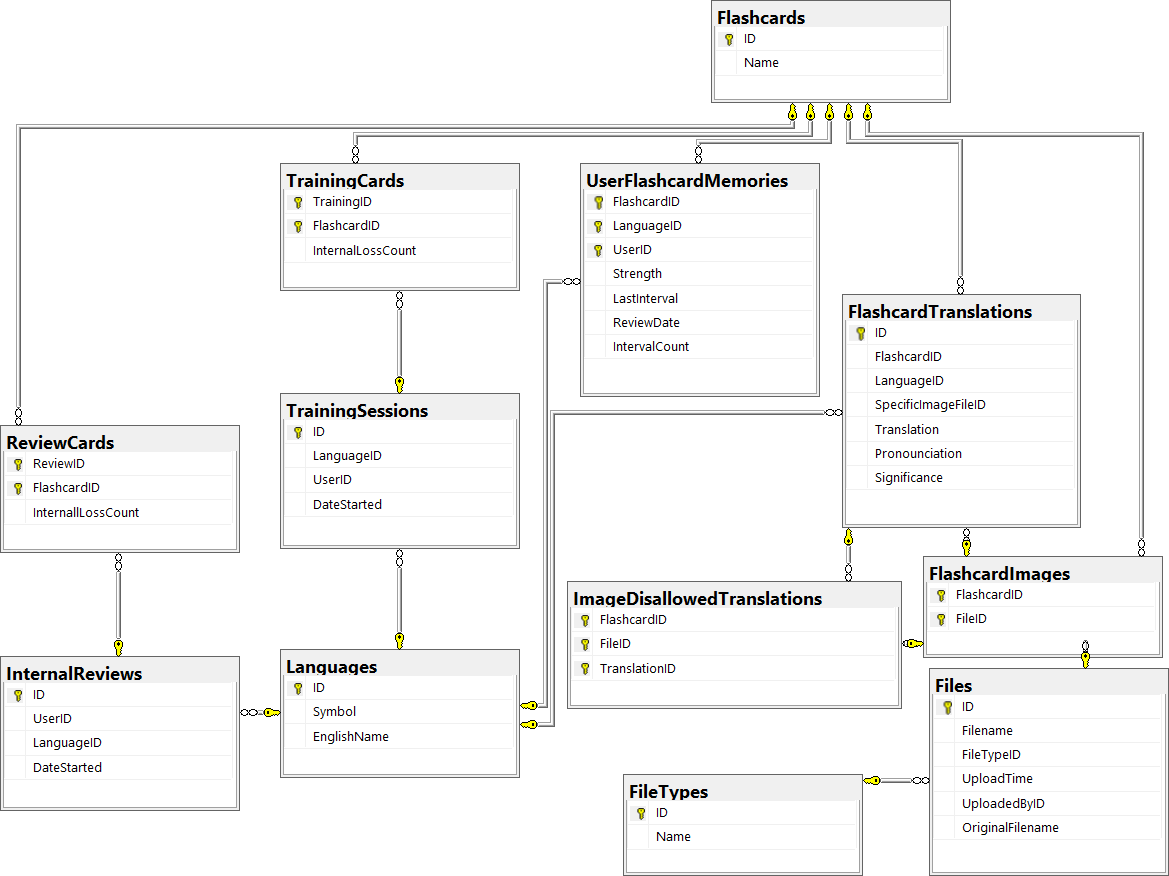
\includegraphics[width=\textwidth]{images/erd.png}
  \captionof{figure}{Diagram ERD bazy danych.}
\end{center}
\end{landscape}


\subsection{Informacje dodane przez ASP.NET MVC}

ASP.NET dostarcza bibliotekę Identity, za której pomocą można łatwo wdrożyć operacje logowania, rejestracji oraz obsługi sesji dla użytkowników. Domyślnie Identity używa lokalnej bazy sqlite\footnote{Baza danych, która operuje na danym pliku binarnym w celu używania bazy danych bez konieczności posiadania dodatkowego serwera.} w celu zapisu informacji o użytkownikach. Aby używać bazy danych SQL należy zmienić connection string, który wykorzystuje biblioteka. Po takiej zmianie zostaną utworzone automatycznie tabele odpowiedzialne za przechowywane informacji o użytkownikach.

\begin{minipage}{\linewidth}
\begin{lstlisting}[
frame=single, numbers=none,captionpos=b, 
caption={Connection string dla biblioteki Identity.}]
<add name="IdentityConnection" connectionString="Data Source=DESKTOP-8H0EDBL\DAMIANSQL;Initial Catalog=Flashcards;Integrated Security=True;MultipleActiveResultSets=True;Connect Timeout=120;" providerName="System.Data.SqlClient" />

\end{lstlisting}
\end{minipage}

Identity dodaje następujące tabele do projektu:
\begin{itemize}
	\item \textunderscore\textunderscore MigrationHistory
	\item AspNetRoles
	\item AspNetUserClaims
	\item AspNetUserLogins
	\item AspNetUserRoles
	\item AspNetUsers\footnote{Tylko ta tabela znalazła się na diagramie ERD}
\end{itemize}

\newpage
\begin{center}
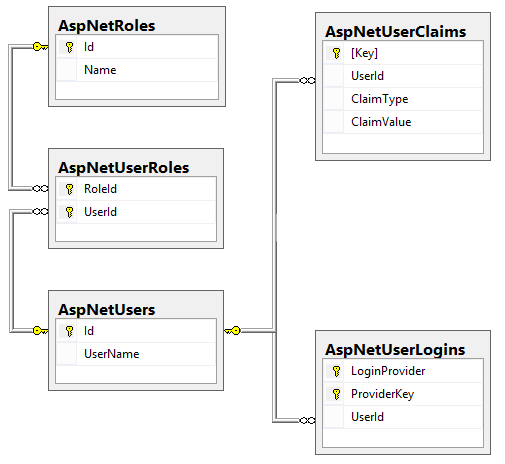
\includegraphics{images/identity.png}
\captionof{figure}{Diagram ERD ASP.NET Identity}
\end{center}


\textunderscore\textunderscore MigrationHistory zawiera informacje stworzone w wyniku migracji z danego rozwiązania bazodanego do innego. W przypadku tego projektu są tutaj zawarte informacje o zmianie domyślnej bazy sqlite na Microsoft SQL Server.

AspNetRoles przechowuje dane o tym jakie role mogą zostać przypisane do użytkowników

AspNetUserClaims zawiera żądania dostępu do konta danego użytkownika. Nie jest ona wykorzystywana w tym projekcie.

AspNetUserLogins zawiera informacje o loginach dla danych użytkowników, za pomocą których mogą się logować na swoje konto.

Wewnątrz tabeli AspNetUserRoles znajdują się informacje o przypisaniu użytkownika do danej roli.

AspNetUsers przechowuje informacje o użytkowniku.

\vspace{5mm}

Wartym uwagi jest fakt, iż biblioteka Identity przechowuje identyfikatory w postaci ciągu 128 znakowego.

\todo[inline]{Jak to jest tworzone}
 
\subsection{Obsługa treningu}

Za obsługę treningu odpowiadają tabele:

\begin{itemize}
	\item TrainingSessions
	\item TrainingCards
\end{itemize}

TrainingSessions przechowuje informacje o danej sesji treningowej pod którą podpięte są aktualnie nauczane karty poprzez tabelę TrainingCards. Połączenie odbywa się za pomocą relacji jeden do wielu.

\subsection{Obsługa powtórki}

Tabele wewnątrz których znajdują się informacje o powtórce to:

\begin{itemize}
	\item InternalReviews
	\item ReviewCards
\end{itemize}

Internal Reviews zawiera informacje o aktualnej powtórce dla danego użytkownika podczas gdy ReviewCards zawierają fiszki przynależąc do danej powtórki. Połączenie odbywa się za pomocą relacji jeden do wielu.

\subsection{Informacje o Fiszkach}

Informacje o fiszkach są przechowywane w tabelach:

\begin{itemize}
	\item Flashcards
	\item FlashcardTranslations
	\item FlashcardImages
	\item ImageDisallowedTranslations
\end{itemize}

Pierwsza z tabel zawiera Identyfikator danej fiszki wraz z jej nazwą angielską, która jest wykorzystywana w narzędziach administratorskich. Dla tej tabeli został stworzony unikalny indeks dla pola Name. Za pośrednictwem tego pola jest zrobione wyszukiwane wewnątrz narzędzi administratorskich, więc przyczynia się to do zwiększenia wydajności zapytań. Dodatkowo, ważne jest to, aby fiszki miały unikalną nazwę systemową, aby mogły być rozróżnialne przez administratora.

FlashcardsTranslations zawiera informacje o tłumaczeniach dla danej fiszki w danym języku. Posiada jeden indeks dla pól FlashcardID i LanguageID. Ta decyzja umotywowana jest faktem zwiększenia szybkości zwracanych zapytań. Program bardzo często będzie wyszukiwał translacji dla danej fiszki według języka i jej identyfikatora.

FlashcardImages zawiera informacje o tym jaki zuploadowany plik jest dopisany dla danej fiszki. Informacja o tym jaki to jest plik i gdzie się znajduje jest zawarta w tabeli Files.

Czasami może się zdarzyć, iż dany obrazek nie oddaje w sposób precyzyjny danego tłumaczenia. Z tego powodu powstała tabela ImageDisallowedTranslations, która określa dla jakiego tłumaczenia dany obrazek nie może zostać użyty.

\subsection{Upload plików}
\label{subsec:uploadFiles}
Wszystkie informacje o zuploadowanych plikach na serwer są określone przez tabele:

\begin{itemize}
	\item Files
	\item FileTypes
\end{itemize}

Tabel Files zawiera informacje o zuploadowanym pliku. Warto tutaj zwrócić uwagę na to, iż nie jest tutaj przechowywana bezwzględna ścieżka do pliku, lecz jedynie jego nazwa wewnątrz kolumny Filename. Określenie dokładnej ścieżki odbywa się z pomocą typu uploadu, który jest określony przez FileTypeID.

Tabela FileTypes jest słownikiem zawierającym nazwę i identyfikator danego typu pliku.




\section{Integracja Scala.js z ASP.NET MVC}
 
Visual studio aktualnie nie posiada żadnego wsparcia dla scali.js\cite{ScalaNoSupport}. Dodatkowo wyniki wyszukiwania w google pod hasłem "Visual studio scala.js"\cite{ScalaNoSupportGoogle} nie zwracają żadnych zapytań. Można więc domniemywać, iż ta praca przeciera niejako szlak podczas prób połączenia tych 2 technologii.
 
W związku z powyższym pierwszą decyzją jaka powinna zostać podjęta podczas tworzenia takiego połączenia to nie używanie środowiska Visual Studio do pisania kodu Scali. Jest ono całkowicie niedostosowane do tego celu. Wewnątrz tej pracy jest używane środowisko \textbf{IntelliJ IDEA}, jednakże można w tym celu użyć każdego innego dowolnego programu (Przy mniejszych programach wystarczy nawet sam edytor tekstowy i linia poleceń).

Projekt Scali.js został utworzony w katalogu ./Scripts/scala \footnote{./ jest katalogiem głównym projektu ASP.NET MVC} z ustawienia build.sbt takimi jak na listingu \ref{lst:scalasbt}.

Mając tak przygotowany projekt oraz zakładając, iż mamy już kompilowalny kod, który może zostać użyty na stronie, musimy przygotować go do wdrożenia w kod .cshtml naszej strony. Wpierw w tym celu przygotujemy paczkę skryptową (po ang. ScriptBundle), która będzie dodana przez ASP.NET MVC na stronie.
Należy to zrobić wewnątrz pliku \textbf{BundleConfig.cs} w projekcie ASP.NET MVC. Kod zastosowany w projekcie jest widoczny na listingu \ref{lst:bundles}.

\begin{minipage}{\linewidth}
\begin{lstlisting}[label=lst:bundles,
frame=single, numbers=none,captionpos=b, 
caption={Dodanie paczek ze skryptami dla BundleConfig.}]
bundles.Add(new ScriptBundle("~/bundles/scalaDependencies").Include(
"~/Scripts/scala/target/scala-2.12/flashcards-jsdeps.js"
));

bundles.Add(new ScriptBundle("~/bundles/scala").Include(
"~/Scripts/scala/target/scala-2.12/flashcards-fastopt.js"
));
\end{lstlisting}
\end{minipage}

Następnie możemy użyć tych paczek wewnątrz kodu .cshtml strony za pomocą instrukcji \textbf{Scripts.Render(''~/bundles/scalaDependencies'')} i \textbf{@Scripts.Render(''~/bundles/scala'')}.

\subsection{Uruchamianie skryptu}

Cały kod Scala.js został podzielony logicznie na pojedyncze klasy, gdzie każda z klas odpowiada danemu widokowi bądź małej grupce widoków. Po stworzeniu takowej struktury nasuwa się następujące pytanie: jak należy zrobić logikę, która jest odpowiedzialna za uruchamianie tych klas?

Wewnątrz projektu zastosowano bardzo prostą metodę, która polegała na utworzeniu klasy Main, która zawierała metodę Init możliwą do uruchomienia z poziomu kodu JavaScript. Funkcja ta przyjmowała zmienną znakową, która zawierała nazwę modułu, który powinien zostać uruchomiony w ramach danej strony. Wykorzystano tutaj instrukcję switch, która w zależności od parametru powodowała uruchomienie metody run obiektu danej klasy.

\begin{minipage}{\linewidth}
\begin{lstlisting}[label=lst:bundles,
frame=single, numbers=none,captionpos=b, 
caption={Dodanie paczek ze skryptami dla BundleConfig.}]
@JSExportTopLevel("InitFlashcard")
//JsExport w tym przypadku informuje o tym, iż ta funkcja powinna być możliwa do wywołania z poziomu JavaScript pod nazwą InitFlashcard.
  def Init(moduleName: String): Unit =
  {
    moduleName match
      {
      case "Management.Index" => new  Flashcards.Management.Index().Run()
      case "Management.EditFlashcard" => new  Flashcards.Management.EditFlashcard().Run()
      case "Training.Question" => new Flashcards.Questions.TrainingQuestion().Run()
      case "Review.Question" => new Flashcards.Questions.ReviewQuestion().Run()
    }
  }
\end{lstlisting}
\end{minipage}

Nie jest to rozwiązanie satysfakcjonujące. Rozwiązanie idealne polegałoby na użycie mechanizmu refleksji (który jest niedostępny wewnątrz Scala.js), bądź podobnym, który na podstawie ciągu znakowego byłby w stanie uruchomić daną klasę bez potrzeby pisania przez programistę osobnej logiki uruchamiania kodu dla każdej z klas.

\section{Implementacje niektórych rozwiązań}

\subsection{Sesja użytkownika}

Po stronie aplikacji ASP.NET MVC dla danego użytkownika zawsze jest podpięta sesja użytkownika, którą identyfikuje się po ciasteczku umieszczonym po stronie przeglądarki. Cały mechanizm zarządzania sesją został umieszczony wewnątrz serwisu \textbf{SessionService}. Wewnątrz sesji zostały umieszczone dane o:

\begin{itemize}
	\item Aktualnie wybranym języku.
	\item Aktualnie zalogowanym użytkowniku. (Jeśli użytkownik był zalogowany)
	\item Aktywnym treningu. (Jeśli użytkownik był zalogowany)
	\item Aktywnej powtórce. (Jeśli użytkownik był zalogowany)
\end{itemize}

Informacja o wybranym języku decydowała o tym w jakim języku powinny odbywać się treningi i powtórzenia. 
Dane aktualnego użytkownika obejmowały jego ID oraz nazwę użytkownika. Były to dane, które bardzo często były używane, dlatego umieszczono je wewnątrz sesji, aby nie pobierać ich z bazy danych.

Dane o aktywnym treningu oraz powtórce umożliwiały sprawne zarządzanie kolejką bez potrzeby dokładnego odwzorowania kolejki po stronie bazy danych. Zmniejszyło to poziom skomplikowania trybu nauczania.

\begin{minipage}{\linewidth}
\begin{lstlisting}[
frame=single, numbers=none,captionpos=b, 
caption={Metody użyte do zapisu i odczytu danych wewnątrz sesji.}]
public static void SetValue(object value, [CallerMemberName] string name = "")
{
	HttpContext.Current.Session[name] = value;
}

public static T GetValue<T>([CallerMemberName] string name = "")
	where T : class
{
	if (HttpContext.Current.Session[name] == null)
		return null;

	return (T)HttpContext.Current.Session[name];
}
\end{lstlisting}
\end{minipage}

\subsection{Kolejka pytań}

Przechowuje informację, w jakiej kolejności pojawiać się będą fiszki, z których użytkownik ma być odpytywany w trakcie nauki. Należy rozróżnić 2 różne kolejki pytań znajdujące się w aplikacji dla każdego z etapów nauki. Jednym z nich jest kolejka znajdująca się wewnątrz sesji użytkownika, nad którą aplikacja ma najłatwiejszą kontrolę i druga, przechowywana po stronie bazy danych, do której poszczególnych elementów aplikacja odwołuje się poprzez repozytoria. 

\subsubsection{Trening}

Algorytm na samym początku treningu pobiera 5 losowych kart i wstawia je do kolejki wewnątrz sesji użytkownika jako Listę obiektów \textbf{TrainingCardInfo}. Te same fiszki zostają wstawione także po stronie bazy danych do tabeli \textbf{TrainingCards}. 

W przypadku niepoprawnej odpowiedzi licznik przegranych jest tak samo uaktualniany wewnątrz sesji, jak i wewnątrz bazy danych. Karta na początku kolejki wewnątrz sesji jest przesuwana na jej koniec.

Usunięcie karty na skutek poprawnej odpowiedzi usuwa informację o obiekcie z sesji, jak i z bazy danych. Dodawana jest przy tym nowa fiszka do sesji, jak i do bazy danych, tak aby w kolejce znajdowało się maksymalnie 5 kart. Jeśli nie ma żadnych nowych przedmiotów do nauczenia się to do kolejki nie są dodawane nowe karty.

W przypadku utraty sesji (na przykład na skutek przelogowania się użytkownika) program stara się przywrócić sesję treningową dla użytkownika. Dokładna kolejność kolejki nie zostanie zachowana. Karty w kolejce zostaną ułożone rosnąco według ilości niepoprawnych odpowiedzi, które zostały zapamiętane.

\subsubsection{Powtórka}

Powtórka działa analogicznie do treningu z kilkoma różnicami:

\begin{itemize}
	\item Przedmiotów wewnątrz kolejki jest maksymalnie 30, a nie 5.
	\item Używana jest lista obiektów \textbf{ReviewCardInfo} i tabela \textbf{ReviewCards}.
	\item W wypadku niepowodzenia fiszka nie jest wstawiana na koniec kolejki, lecz wewnątrz danego przedziału, który został opisany w sekcji \ref{sub:powtorka}.
\end{itemize}

Utrata dokładnej kolejności fiszek w przypadku straty sesji jest bardziej bolesna dla trybu powtórki. Pomimo tego nie jest to problem dla aplikacji, ponieważ utrata sesji odbywa się bardzo rzadko. Dodatkowo użytkownik prawdopodobnie nie zorientowałby się, że kolejność została wymieszana, ponieważ interfejs nie informuje o aktualnym stanie kolejki.

\subsection{Podobieństwo wyrazów}

Podobieństwo wyrazów opisane wewnątrz sekcji \ref{sec:similarity} zostało zaimplementowane w klasie \textbf{LevenshteinSimilarity} implementującej interfejs \textbf{ISimilarityAlgorithm}. Klasa ta jest instancjonowana tylko w jednym miejscu w programie - wewnątrz klasy \textbf{QuestionService}, której zadaniem jest sprawdzenie poprawności odpowiedzi. Ma to na celu umożliwienie łatwej podmiany algorytmu, jeśli zaimplementowany zostanie interfejs \textbf{ISimilarityAlgorithm} przez inną klasę.

\begin{minipage}{\linewidth}
\begin{lstlisting}[
frame=single, numbers=none,captionpos=b, 
caption={Interfejs dla klas obliczających podobieństwo wyrazów.}]
namespace Common.Words.Similiraties
{
    public interface ISimilarityAlgorithm
    {
    	//Metoda powinna zwrócić liczbę z zakresu 0-1 jako miarę podobieństwa między podanymi wyrazami.
        double CalculateSimilarity(string original, string compared);
    }
}
\end{lstlisting}
\end{minipage}


\subsection{Atrapy obiektów}

Wewnątrz programu zastosowano framework Moq do tworzenia atrap obiektów. Niestety to nie zawsze wystarcza. Szczególnie w wypadku gdy potrzebna jest atrapa obiektu bazodanowego, którego wartości są przynajmniej poprawne i wypełnione. Z tego też powodu powstał interfejs \textbf{IDummyCreator<T>}, którego zadaniem jest stworzenie atrapy obiektu "T". Odbywa się to za pomocą metody \textbf{Create}, która zawsze po wywołaniu ma zwrócić pełnoprawny obiekt. 


\begin{minipage}{\linewidth}
\begin{lstlisting}[label={lst:dummyCreator},
frame=single, numbers=none,captionpos=b, 
caption={Przykład kreatora atrap na podstawie LanguageDummyCreator.}]
public class LanguageDummyCreator : IDummyCreator<Language>
{
	private static UniqueIDGenerator uniqueID = new UniqueIDGenerator();
	private Language language;
	public LanguageDummyCreator() { language = create(); }
	{   return new Language()
		{
			ID = uniqueID,
			EnglishName = RandomGenerator.GenerateString(10),
			Symbol = RandomGenerator.GenerateString(2)
		};
	}
	public Language Create()
	{
		var temp = language;
		language = create();
		return temp;
	}
}
\end{lstlisting}
\end{minipage}

\subsubsection{Unikalne identyfikatory}

Powyższe atrapy bazodanowe byłyby całkowicie nieprawidłowe, gdyby nie miały unikalnych identyfikatorów. Wiele metod bazuje na założeniu unikalności identyfikatorów. Nawet w testach jednostkowych brak tej unikalności może być powodem błędów.

W celu rozwiązania tego problemu stworzono \textbf{UniqueIDGenerator}, którego zadaniem jest wygenerować unikalny identyfikator dla danej instancji tej klasy. Jego działanie jest bardzo proste i polega na inkrementowaniu licznika.

Przykład użycia tej klasy można zobaczyć na listingu \ref{lst:dummyCreator}.


\begin{minipage}{\linewidth}
\begin{lstlisting}[
frame=single, numbers=none,captionpos=b, 
caption={Implementacja UniqueIDGenerator.}]
public class UniqueIDGenerator
{
	private int _uniqueID = 0;
	public int UniqueID { get { return _uniqueID++; } }
	public static implicit operator int(UniqueIDGenerator generator)
	{
		return generator.UniqueID;
	}
}
\end{lstlisting}
\end{minipage}

\subsubsection{Enumator}

W projektach bazodanowych bardzo często dochodzi do sytuacji w których są używane tabele słownikowe. Przykładem takiej tabeli może być tabela \textbf{FileTypes}, która zawiera identyfikator i nazwę pliku. 

Bardzo wygodnym rozwiązaniem przy takich tabelach jest utworzenie typu enum, który zawiera wszystkie dozwolone wartości jakie mogą być wykorzystywane przez program dla danej tabeli słownikowej. Wprowadza to statyczne sprawdzenie czy użyliśmy dobrej wartości, ponieważ mamy tylko ich skromny zakres dostępny z enuma. Kompilator powiadomi nas o tym, jeśli chcemy użyć czegoś co nie istnieje.

Dodatkowo możemy wykorzystać Intellisense\footnote{Jest to narzędzie podpowiadające składnię podczas pisania kodu.} do podpowiadania nam dostępnych wartości.

\vspace{5mm}

Niestety takie rozwiązanie ma jeden i to ważny problem. Bardzo ciężko jest jednocześnie edytować tabelę i enuma występującego w kodzie. Bez żadnego narzędzia programista zawsze musi pamiętać, iż przy edycji jednego zawsze musi zostać zedytowana druga rzecz. Może to doprowadzić do trudnych do wykrycia błędów.

Z tego też powodu stworzyłem typ \textbf{Enumator}, który na podstawie danego Enuma wypełnia daną tabelę za pomocą Entity Frameworka odpowiednimi wartościami. 	
Typ ten potrafi za pomocą metody \textbf{CreateNewIfAble} stworzyć nieistniejące rekordy dla danych kluczy głównych w tabeli. W domyślnej wersji na podstawie wszystkich wartości z danego enuma tworzy wykryte nieistniejące rekordy przypisując im odpowiednie wartości poprzez właściwości \textbf{ID} i \textbf{Name}.

\begin{minipage}{\linewidth}
\begin{lstlisting}[
frame=single, numbers=none,captionpos=b, 
caption={Metoda CreateNewIfAble.}]
public Enumator<TEntity, TEnum, TContext> CreateNewIfAble()
{
	var all = repository.GetAll();

	foreach (TEnum val in Enum.GetValues(typeof(TEnum)).Cast<TEnum>())
	{
		if (all.Any(entity => ((dynamic)entity).ID == (int)((dynamic)val)))
			continue;

		string name = val.ToString();
		int value = (int)((dynamic)val);

		TEntity newEntity = new TEntity();
		((dynamic)newEntity).Name = name;
		((dynamic)newEntity).ID = value;

		repository.Add(newEntity);
	}

	repository.SaveChanges();
	return this;
}
\end{lstlisting}
\end{minipage}

\subsubsection{Upload plików}

Wewnątrz aplikacji zaimplementowano system uploadu plików oparty o rozwiązania dostarczane przez ASP.NET MVC. 

Zostało to wykorzystane przy dodawaniu nowego obrazka do danej fiszki.
W tym celu stworzono formularz, wewnątrz którego dodano dwa elementy \textbf{input}. Jeden ukryty informujący o ID karty i drugi, wewnątrz którego była przechowywana informacja o uploadowanym pliku. W celu poprawnego przesyłu danych przez formularz należy użyć elementu \textbf{form}, który do przesyłu danych używa formatu MIME. Można to osiągnąć poprzez ustawienie atrybutowi \textbf{enctype} wartości \textbf{multipart/form-data}.

Wewnątrz akcji odpowiedzialnej za upload pliku należy użyć typu \textbf{HttpPostedFileBase} jako argumentu, za którego pośrednictwem przychodzi do nas informacja o zuploadowanym pliku. Typ ten zawiera wszystkie informacje o zuploadowanym pliku. 

Następnie wykorzystywany jest serwis \textbf{FlashcardImageService}, którego zadaniem jest sprawdzenie, czy możliwy jest upload danego obrazka. W przypadku, gdy serwis stwierdzi taką możliwość, jest uruchamiana procedura uploadu pliku za pośrednictwem serwisu \textbf{UploadService}.

Po stronie serwera zostanie utworzony unikalny plik o tym samym rozszerzeniu co rozszerzenie uploadowanego pliku. Nazwa tego pliku będzie generowana na podstawie metody \textbf{Path.GetRandomFileName}, która jest dostarczana przez .NET Framework. Plik zostanie zuploadowany w miejscu wskazanym przez klasę \textbf{UploadLocation} na podstawie rodzaju uploadu (w tym wypadku typem uploadu jest upload obrazków).

Po zakończeniu procedury nowy obrazek może być od razu wykorzystywany przez użytkownika.

\begin{minipage}{\linewidth}
\begin{lstlisting}[
frame=single, numbers=none,captionpos=b, 
caption={Metoda UploadNewImage wewnątrz FlashcardImageService, która uploaduje plik z obrazkiem.}]
public void UploadNewImage(Flashcard flashcard, HttpPostedFileBase file, string userID)
        {
            var dbFile = uploadService.Upload(file, userID, FileTypeEnum.FlashcardImage);

            unit.FlashcardImageRepository.Add(new FlashcardImage()
            {
                FileID = dbFile.ID,
                FlashcardID = flashcard.ID
            });
            
            unit.FlashcardImageRepository.SaveChanges();
        }
\end{lstlisting}
\end{minipage}
